\documentclass{beamer}
\usepackage[british]{babel}
\usepackage{graphicx}

\usetheme{metropolis}

\title{Networking in Unity}
\subtitle{Workshop for COMP280}
\author{Joseph Walton-Rivers \& Archie Andrews}

\begin{document}
	\begin{frame}
		\maketitle
	\end{frame}

	\begin{frame}
		\frametitle{Multi-player Games}
		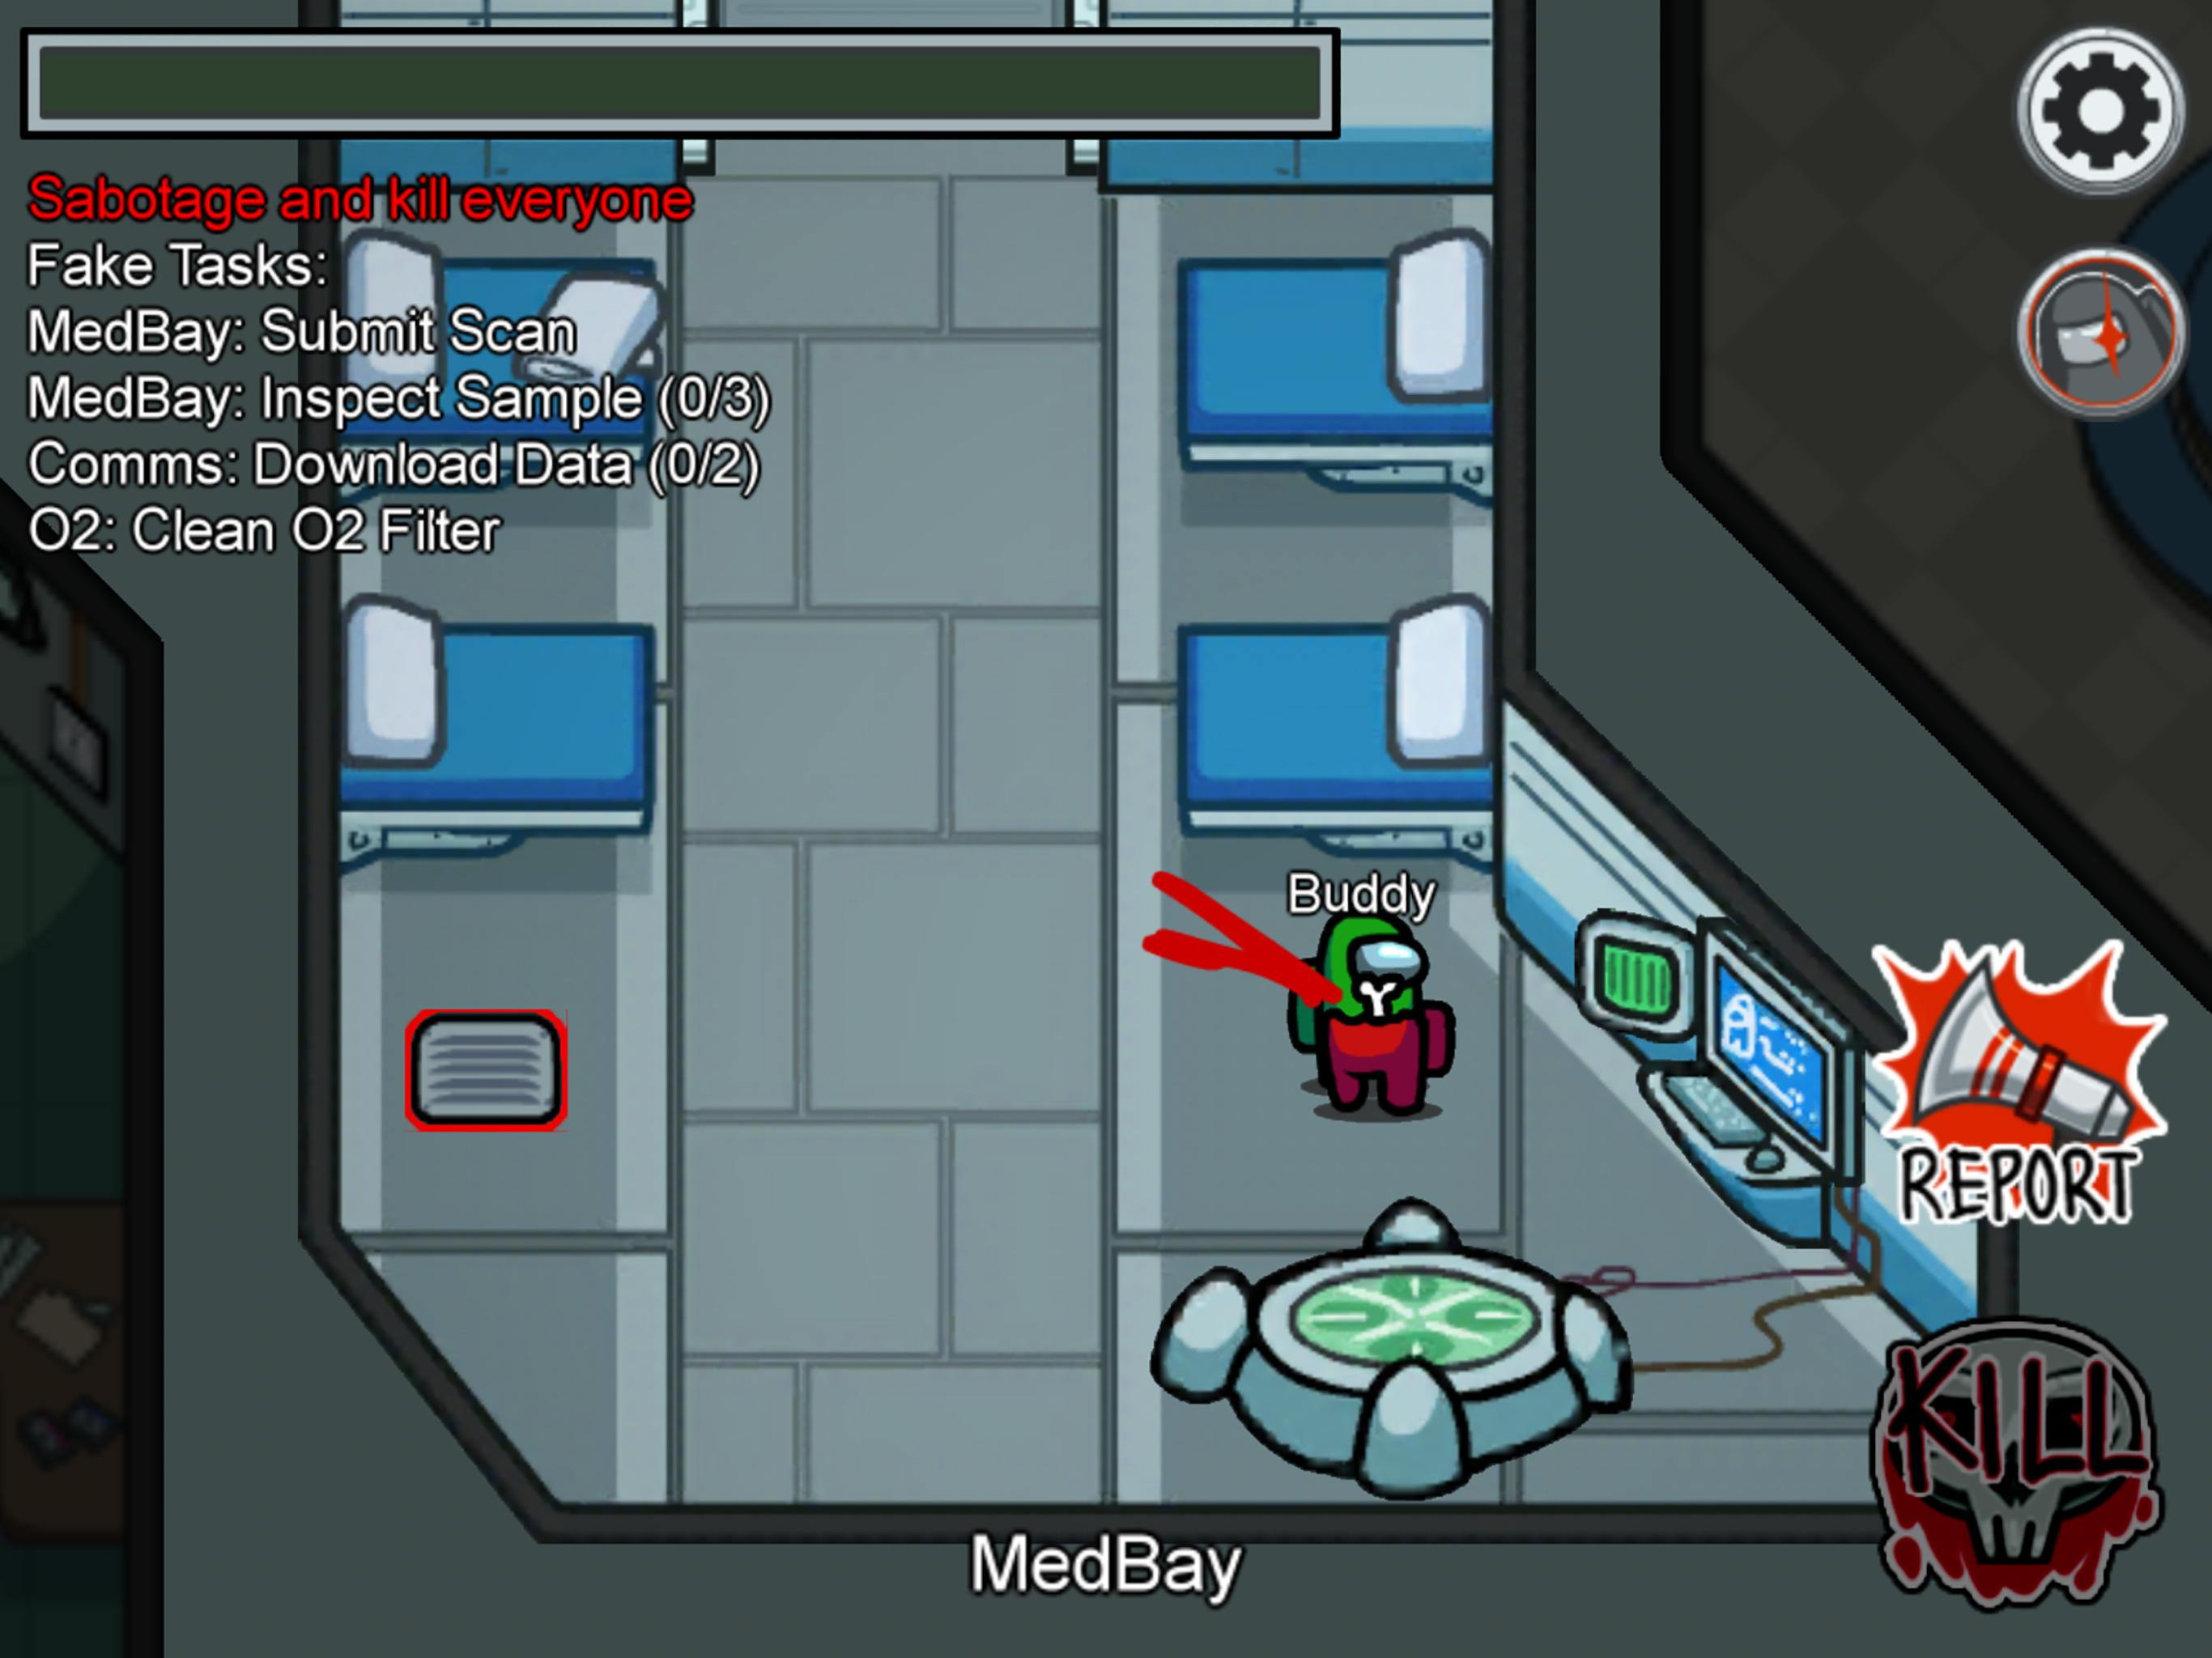
\includegraphics[width=\textwidth]{game_amungus}
	\end{frame}

	\begin{frame}
		\frametitle{Multi-player Games}
		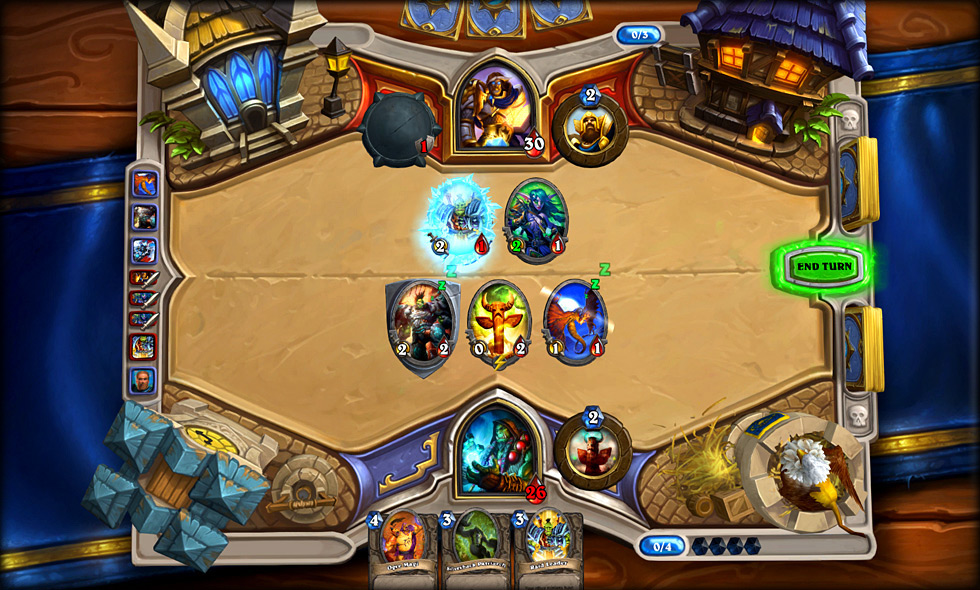
\includegraphics[width=\textwidth]{game_harthstone}
	\end{frame}

	\begin{frame}
		\frametitle{A word of caution}
		
		\begin{itemize}
			\item I've chosen both my examples carefully
			\item Note the number of players
			\item (they're not MMOs or Battle Royale games!)
			\item Multi-player is hard, more players makes life harder!
			\item So stick to smaller games for now...
		\end{itemize}
		
	\end{frame}

	\section{Context}
	
	\begin{frame}
		\frametitle{Basic Architecture}
		
		\begin{itemize}
			\item We'll be considering a client-server model for this session
			\item True peer-to-peer for games are tricky
			\item Note: a `server' could be one of the players
			\item It will be in our examples
		\end{itemize}
	
	\end{frame}

	\begin{frame}
		\frametitle{State}
		
		\begin{itemize}
			\item Before talk about networking, we should probably talk about the notion of \textit{state}
			\item \textit{State} is the information that makes up your game world \begin{itemize}
				\item A door's state might be if it's position, and if it's open or closed
				\item A player's state might be their position, how much health they have, what items they are carrying, etc...
			\end{itemize}
		\end{itemize}
	\end{frame}

	\begin{frame}
		\frametitle{The basic idea}
		
		\begin{itemize}
			\item We want to make sure that the game's \textit{state} is the same between users
			\item We can do this by ensuring that when something changes, we tell other players
			\item We usually do this by sending messages to an intermediary (a server) that then tells all the other players
		\end{itemize}
	
	\end{frame}

	\begin{frame}
		\frametitle{Conflicts}
		
		\begin{itemize}
			\item We're playing a game that features the ability to pick up objects
			\item Two players \textbf{both} try to pick up the same object at the same time
			\item Who has the object?
		\end{itemize}
	\end{frame}

	\begin{frame}
		\frametitle{Basic Overview}
		
		A simplified view of networking for games:
		
		\begin{enumerate}
			\item Clients send request(s) / update(s) to the server
			\item The server processes the request
			\item The server lets the client(s) know the result
			\item The clients update their state to match
		\end{enumerate}
	
		nb. sometimes changes can happen on their own
	\end{frame}
	
	\begin{frame}
		\frametitle{Protocol}
		
		\begin{itemize}
			\item The \textbf{Protocol} is the format of the messages between the clients and the server
			\item Can be / is usually game-specific
			\item Can be stateful (eg, move can only be sent after login)
		\end{itemize}
	
		Examples: \href{https://minecraft.gamepedia.com/Classic_server_protocol}{Minecraft 'classic' protocol}, \href{https://www.amazon.com/Designing-Virtual-Worlds-Richard-Bartle/dp/0131018167}{Designing Virtual Worlds},
		\href{https://www.youtube.com/watch?v=W3aieHjyNvw}{Overwatch Netcode Talk}
		% https://rsps.fandom.com/wiki/317_Protocol - not sure I should mention this one...
	\end{frame}
	
	\section{Today's activities}
	
	\begin{frame}
		\frametitle{By the end of today}
		
		\begin{itemize}
			\item You should have a good understanding of the principles behind networking in Unity
			\item You should understand how to use Forge to build games
			\item You should have a simplistic multi player scene
		\end{itemize}
	\end{frame}
	
	\begin{frame}
		\frametitle{Cubes!}
		
		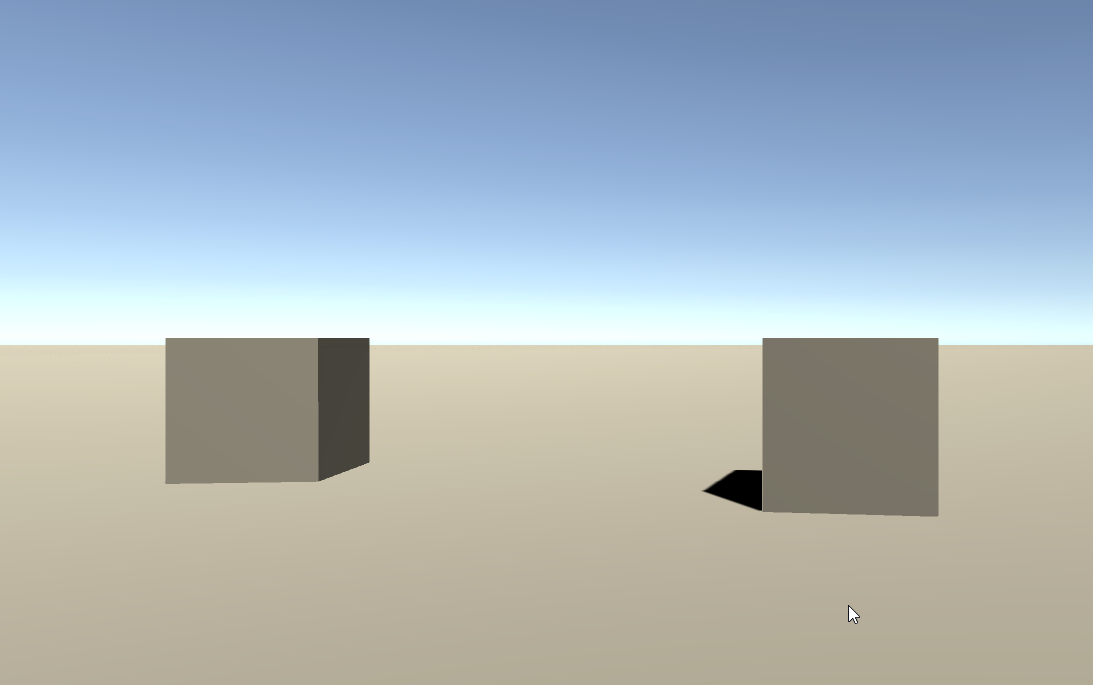
\includegraphics{unity_twocubes}
	\end{frame}
	
	\begin{frame}
		\frametitle{A simple networked application}
		
		\begin{itemize}
			\item You can find the instructions for today on the learning space
			\item We'll be doing three (possibly 4 if you have time) activities to teach is the \textbf{Basics} of networking in Unity
			\item My example game is a little bare bones - that's so you can customise it 
		\end{itemize}
	\end{frame}

	\begin{frame}
		\frametitle{See Learning Space}
		
		\begin{center}
			Activity sheet on learning space
		\end{center}
		
	\end{frame}
	
	\begin{frame}
		\frametitle{Activity 1 - Cubes}
		
		\begin{itemize}
			\item Now you should have a working player controller with basic movement
			\item For the next part we'll make the clients have a cube to
			\item Questions?
		\end{itemize}
	\end{frame}
	
	\subsection{Activity 2}
	
	\begin{frame}
		\frametitle{Activity 2 - Two Cubes}
		
		\begin{itemize}
			\item Every connected player should have a cube now
			\item They should be able to move independently
			\item \textbf{possible bug}: updating the transform directly can make physics unhappy 
		\end{itemize}
	\end{frame}
	
	\subsection{Activity 3}
	
	\begin{frame}
		\frametitle{Activity 3 - RPC }
		
		\begin{itemize}
			\item We've now seen how we can call methods on other peoples machines
			\item Very useful for dealing with anything that'd not happening every frame
			\item Careful about who can do what - possible security problems
		\end{itemize}
	
	\end{frame}

	\begin{frame}
		\frametitle{Activity 4 - sync bugs}
		
		\begin{itemize}
			\item Now we've seen what can happen when we don't sync stuff properly
			\item Question: would we ever want to do stuff on the clients? Why not do it all on the server?
			\item talking point: Rubber banding
		\end{itemize}
		
	\end{frame}
	
	\section{Debrief}
	
	\begin{frame}
		\frametitle{Showcase?}
		
		\begin{center}
			Anyone want to share what they've made?
		\end{center}
	\end{frame}
	
	\begin{frame}
		\frametitle{Networking in Unity}
		
		\begin{itemize}
			\item Today we've built a simple networked application
			\item Syncing, creating objects and RPC are the cornerstones of our networking activities (at least for Unity...)
			\item Play with what you've learnt today and see what you can build!
		\end{itemize}
	
	\end{frame}

\end{document}